\documentclass{article}
\usepackage{parskip}
\usepackage{pdfpages}
\usepackage[margin=.6in]{geometry}
\begin{document}
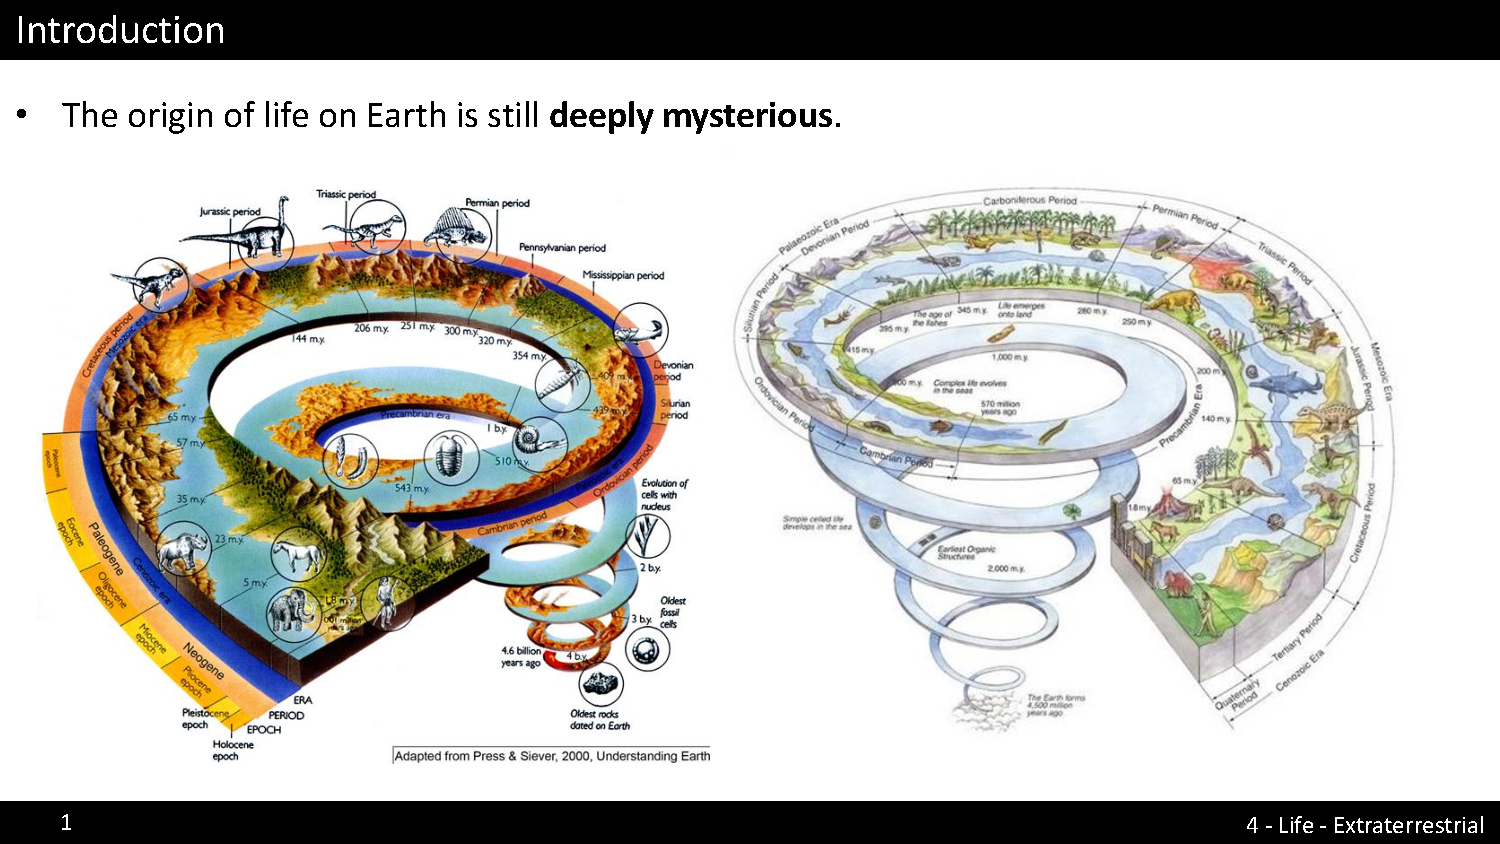
\includepdf[pages=1-3]{slides}
We talked about the ways that life might have occurred on earth. Its very probably that it happened without outside force, which means that it could happen on other planets.

\includepdf[pages=3-6]{slides}
Just remember the shit from astro 101.

\includepdf[pages=7-8]{slides}
The kind of start determines where the habitable zone is, habitable zone is just where liquid water can exist.

\includepdf[pages=9-14]{slides}
Exoplanets are very hard to detect because they only emit reflected light from their sun, but the star is so powerful it hides the planet. We dont really see them, instead we have indirect proof.

The planets subtly alter the stars location due to the effect of gravity and we can see this wobble. The sun should give off perfect light but there are little spots in the atomic spectrum there are tiny particles in the star's atmosphere and we can use these spots to see if the star is red shifted or blue shifted and from this we can see if the star is moving closer or farther from us. This is how we measure the wobble and know how the star is moving. This gives us the mass of the planet. We can use the period of the wobble to know how far the planet from the sun. This will tell us if it is in the habitable zone.

\includepdf[pages=15]{slides}
We can also learn alot about planets that are planar to us.

\includepdf[pages=16]{slides}
\includepdf[pages=17]{slides}
We frequently compare the planet's density to water. We know this because we can get its size and mass. Its crazy what we know.

\includepdf[pages=18]{slides}
The kepler mission was awesome. It brought back a ton of data. For instance this is the orbital time for known planets (we need three sightings for this).11

\includepdf[pages=19]{slides}
Its much easier to see planets that are closer to their star so we have more data on them.

The green band on the second picture shows where liquid water might exist.

\includepdf[pages=20]{slides}
\includepdf[pages=21]{slides}
We recently discovered some very promising planets.
\includepdf[pages=22-27]{slides}

Potential question for assignment = \emph{could life evolve on a water world?}

\includepdf[pages=28-32]{slides}
For life to exist all the laws that we have have to be the same, but these are universal laws so its reasonable.

\includepdf[pages=33-42]{slides}
Life on early basically happened immediately after the late heavy bombardment caused the right conditions. This implies that the transition between chemestry and biology is easier than we think.

\includepdf[pages=43]{slides}
When we looke at the rates of oxygen throughout the history of earth we can see that there have been 5 massive extinctions. Right after these dips we see spikes implying that life comes right back up after the extinction.

\includepdf[pages=44-46]{slides}


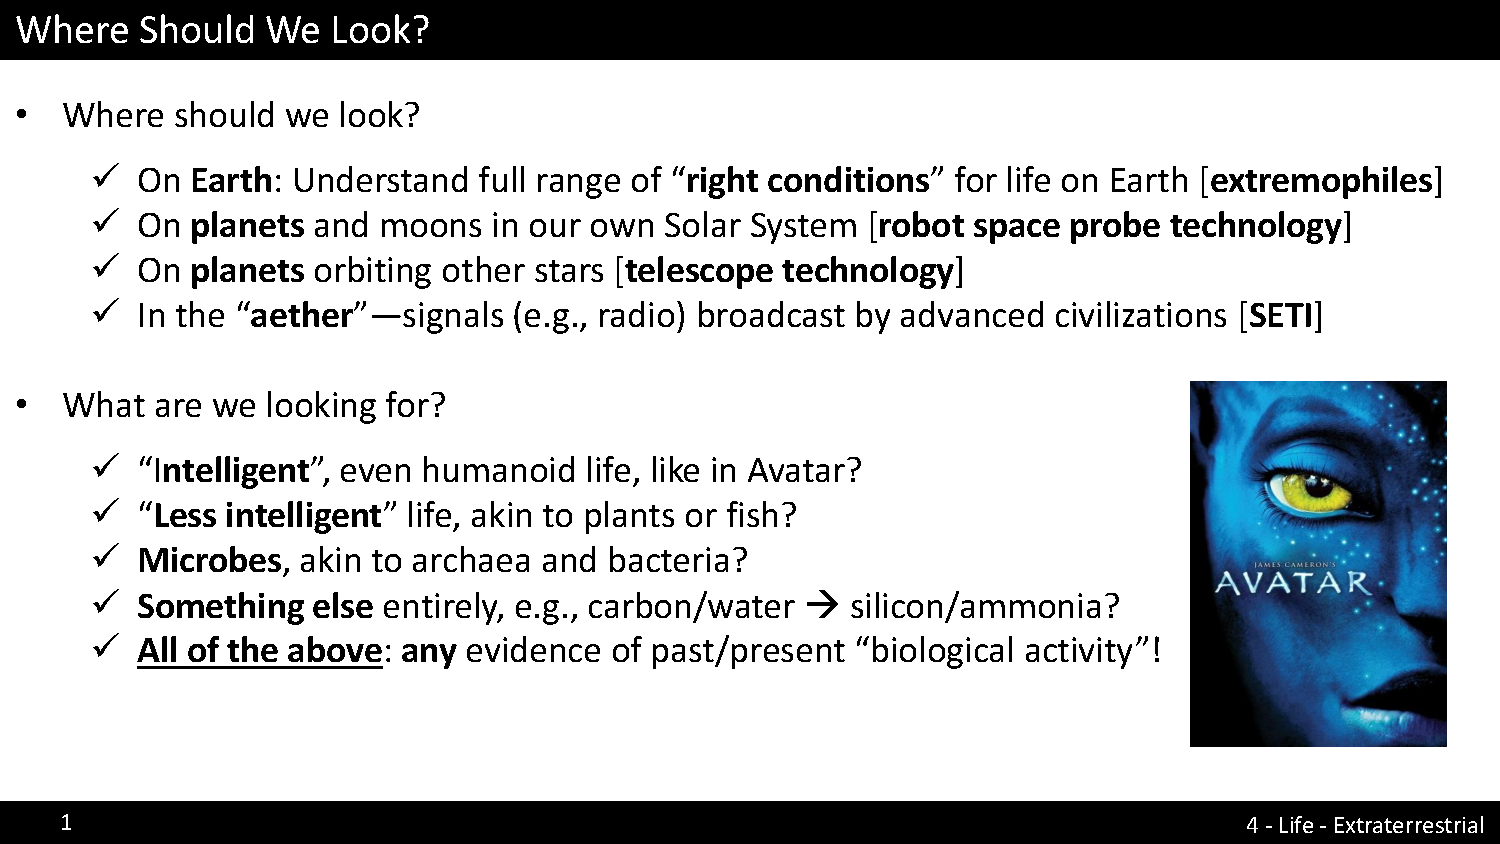
\includepdf[pages=1-2]{slides2}
Its possible that we could have life arrive under different circumstances, using different elements. Life only uses 25/92 of the naturally ocurring elements,

\includepdf[pages=3-4]{slides2}
We need liquid because stuff as to move around to break things down and reform them. They are required for transporting things used in the processes of life. Water in particular is very important because it has many unique properties (is polar for dissolving, made of common elements, is less dense when frozen).

\includepdf[pages=5]{slides2}
If you have life in a cold liquid its metabalism is slower and vice versa.

\includepdf[pages=6]{slides2}
Titan has rocks made out of water and an nitrogen rich atmosphere.

\includepdf[pages=7]{slides2}








\end{document}
